\chapter{Feder}

\section{Definition}

\begin{figure}[h!]
	\centering
	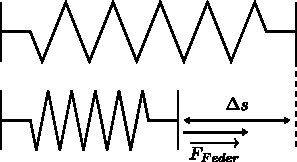
\includegraphics[scale=0.75]{feder-dehnung.pdf}
	\caption{Veranschaulichung der Federdefinition.}
	\label{fig:feder-dehnung}
\end{figure}

\noindent
Eine Feder kann gedrückt oder gezogen werden, wobei eine Kraft $F$ entsteht,
welche proportional zur Dehnung $s$ ist. Die Proportionalität wird durch die
sogenannte Federkonstante $k$ beschrieben. Dies wird auch als Hook'sches
Gesetz bezeichnet.
\[ \boxed{F_{Feder} = k \cdot s} \]

\noindent
Die Richtung der Kraft ist hierbei stets entgegen der Dehnung, d.h. wird die
Feder gestreckt, so zeigt die Kraft zur Feder hin und wird die Feder
gestaucht, so zeigt die Kraft von der Feder weg.

\section{Energie}\label{sec:feder-energie}
Die Energie einer Feder ist definiert als die Federkonstante $k$ multipliziert
mit dem Integral der Dehnung (Weg $\Delta s$ bzw. s).
\begin{figure}[h!]
	\centering
	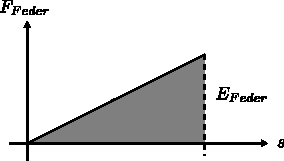
\includegraphics[scale=0.9]{feder-energie.pdf}
	\caption{Energie einer Feder als Fläche dargestellt.}
	\label{fig:feder-energie}
\end{figure}

\[ \boxed{E_{Feder} = k \cdot \int_{s_a}^{s_b} s \cdot ds = \frac{k \cdot s^2}{2}} \] \\

\section{Kombination}
Federn können nicht nur einzeln sondern in Kombinationen vorkommen. Hierbei
werden im speziellen zwei Fälle unterschieden:

\begin{itemize}
	\item Parallele Anordnung von Federn
	\item Serielle Anordnung von Federn
\end{itemize}

\begin{figure}[h!]
	\centering
	\begin{subfigure}[c]{0.45\textwidth}
		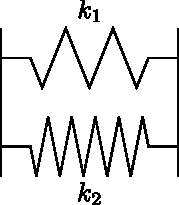
\includegraphics[scale=0.75]{feder-parallel.pdf}
		\caption{Parallele Federanordnung.}
		\label{fig:feder-parallel}
	\end{subfigure}
	\begin{subfigure}[c]{0.45\textwidth}
		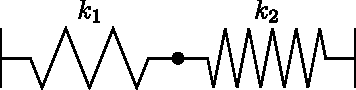
\includegraphics[scale=0.75]{feder-seriell.pdf}
		\caption{Serielle Federanordnung}
		\label{fig:feder-seriell}
	\end{subfigure}
	\caption{Federanordnungen in Vergleich}
	\label{fig:federanordnungen}
\end{figure}

\subsection{Parallele Anordnung}

\noindent
Werden Federn parallel angeordnet, so können die Federkosntanten summiert 
werden.

\[ \boxed{k_{parallel} = \sum_{i=1}^n k_i = k1 + k2 + \dots + k_n} \]

\subsection{Serielle Anordnung}

\noindent
Werden Federn seriell angeordnet, so können die Federkonstanten reziprok 
summiert werden.

\[ \boxed{\frac{1}{k_{seriell}} = \sum_{i=1}^n \frac{1}{k_i} = 
	\frac{1}{k_1} + \frac{1}{k_2} + \dots + \frac{1}{k_n}} \]

\[ \boxed{\frac{E_1}{E_{Total}} = \frac{k_1 \cdot {k_2}^2}{k_1 + k_2}} \]  
\[ \boxed{\frac{E_2}{E_{Total}} = \frac{{k_1}^2 \cdot k_2}{k_1 + k_2}} \]  
\[ \boxed{\frac{E_1}{E_2} = \frac{k_2}{k_1}} \]
\[ \boxed{\frac{E_2}{E_1} = \frac{k_1}{k_2}} \]

\section{Federkonstante}
Die Federkonstante ist eine material- und geometrieabhängige Grösse welche
berechnet werden kann mittels des sogenannten Elastizitätsmoduls $E$, der
Querschnittsfläche $A$ und der neutralen Länge $l_0$.

\[ \boxed{k = \frac{E \cdot A}{l_0}} \]

